\subsection{スマホアプリによるビーコンと実デバイスによるビーコンの併用}

% 語るべき内容
% そもそも文章がガリガリ削ったあとなのでそれの復元
% 技術の解説がない BLEなど
% スマホビーコンの画面が欲しい
% 実装時の流れ ユーザにとってUUIDを意識せずに使えるようにあたりは深掘りできそう


実デバイスによるビーコンはメンバの利便性が低く可用性に問題がある.
可用性とは,メンバの在室情報が長期にわたり継続的に記録される能力と定義する.
実デバイスによるビーコンを利用する場合,高い可用性を維持するにはバッテリ交換に配慮する必要がある.
そこで既存研究ではバッテリ切れが発生した場合,管理者がメンバにSlackを用いて
通知しバッテリ交換を催促していた.
しかし交換されない状況が存在した.
これは通知による催促が不確実かつ即時性がないためである.
通知は一定期間の在室がない場合にバッテリ切れの可能性があると見做して通知している.
そのため通知の正確性が低い上,バッテリ切れに対してタイムラグがある.
また交換作業がメンバに委ねられており,その手間による利便性が低くバッテリ切れの放置が発生した.


上記の問題のアプローチとしてメンバの利便性を向上させるため,スマホアプリによるビーコン動作(以下,スマホビーコン)を行った.
BLEビーコンの代替としてスマートフォンを利用可能にするとバッテリ交換の手間が削減される.
またスマートフォンユーザにとってスマートフォンはコミュニケーションツールとしての用途からバッテリ切れを配慮する傾向が強い.
よって実デバイスによるビーコンと比べてスマホビーコンはバッテリが維持されやすく利便性が向上すると考えた.

スマホビーコンは基本的にバックグラウンドに常駐させる利用法を想定し実装した.
既存研究では,メンバに実デバイスによるビーコンを携帯させ,能動的な記録動作の必要がない.
バックグラウンドに常駐させる方式は実デバイスによるビーコンと同様に能動的な記録動作を必要としないため同等の利便性がある.
スマートフォンの画面表示が可能な利点を利用し,スマートフォンの通知領域に動作状況を表示した.
通知領域への表示はスマホビーコンの動作と連携しており,動作中に表示される.
メンバにとって実デバイスによるビーコンは動作の把握が困難であったが,通知領域への表示により動作の把握が可能になった.
そのためビーコン動作の停止に気が付きやすく,メンバによる再起動が行われた場合,可用性の向上が期待できる.





スマホビーコンのみを利用する場合,様々な状況下でメンバの継続した利用が困難であるため,実デバイスによるビーコンと併用できるシステムとした.
普段から継続的に利用するメンバにとっては,実デバイスによるビーコンは先述の通りバッテリ交換の手間がある.
スマホビーコンはそのようなメンバにとっては,バッテリ交換の手間がないため有用である.
しかしスマホビーコンのインストールに抵抗があるメンバやインストールができないメンバも想定される.
例としてはスマートフォンを所有していないメンバ,スマホビーコンの利用に伴うバッテリ消費が気になるメンバなどが挙げられる.
これらの問題は実デバイスによるビーコンとスマホビーコンのハイブリッド化によって解決できる.
スマホビーコンで利用するUUIDを実デバイスによるビーコンで利用するUUIDと同じ値に設定し同じメンバの在室情報を記録している.
この方法は表1に示す通りスマホビーコンか実デバイスによるビーコンの少なくとも片方を携帯していれば記録できるため継続的にデータを記録する観点から見ても有用である.
% \begin{table}[tbh]
%   \centering
%   \caption{各ビーコンのみ対応時とハイブリッド対応時の比較}
%   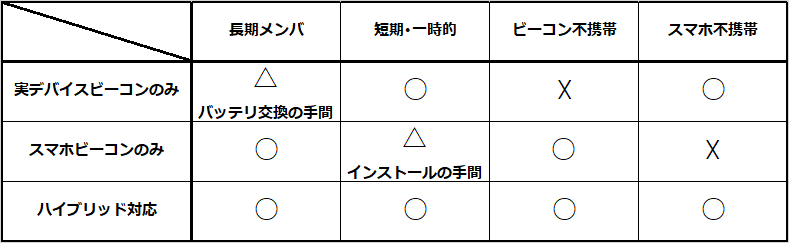
\includegraphics[width=9cm]{image/table.png}
%   \label{multipleBPM}
% \end{table}
\begin{table}[tbh]
    \caption{各ビーコンのみ対応時とハイブリッド対応時の比較}
    \scalebox{0.55}{
        \begin{tabular}{|c|c|c|c|c|}
                \hline
                 & 長期メンバ & 短期・一時的 & スマホ不携帯 & ビーコン不携帯 \\ \hline
                実デバイスビーコンのみ & \begin{tabular}[c]{@{}c@{}}△\\ バッテリ交換の手間\end{tabular} & ○ & ☓ & ○ \\ \hline
                スマホビーコンのみ & ○ & \begin{tabular}[c]{@{}c@{}}△\\ インストールの手間\end{tabular} & ○ & ☓ \\ \hline
                ハイブリッド対応 & ○ & ○ & ○ & ○ \\ \hline
                \end{tabular}
    }
    \label{multipleBPM}
\end{table}

% \begin{table}[tbh]
%     \scalebox{0.25}[0.25]{
%     \begin{tabular}{|c|c|c|c|c|}
%     \hline
%      & 長期メンバ & 短期・一時的 & スマホ不携帯 & ビーコン不携帯 \\ \hline
%     実デバイスのみ & \begin{tabular}[c]{@{}c@{}}△\\ バッテリ交換\end{tabular} & ○ & ☓ & ○ \\ \hline
%     スマホのみ & ○ & \begin{tabular}[c]{@{}c@{}}△\\ インストール\end{tabular} & ○ & ☓ \\ \hline
%     ハイブリッド対応 & ○ & ○ & ○ & ○ \\ \hline
%     \end{tabular}
%     }
%     \end{table}

% chatgptで出した主要技術の解説 流し読みしたところ間違ってる場所はなさそう



あなたは情報科学を学ぶ大学生です.卒業論文を記述するためにAndroid端末におけるBluetooth Low Energyのペリフェラル動作に関する説明文を500文字程度で記述する必要があります.
以下に説明文を記述してください
Bluetooth Low Energy (BLE)は、低消費電力のワイヤレス通信技術です。Android端末では、BLEのペリフェラル動作として、周辺デバイスとの接続をすることができます。

BLEペリフェラルは、通信を受け付ける端末として動作します。アプリケーションからは、GATTプロファイルを使用して、BLEデバイスと通信をすることができます。 GATTプロファイルは、デバイスのサービスやキャラクタリスティックを定義します。

BLEペリフェラル動作を実現するには、Android端末でBLE APIを使用します。これにより、端末をスキャンして周辺のBLEデバイスを検索し、接続を確立し、データの送受信を行うことができます。

BLEは、スマートフォンやタブレットなどの消費者向けデバイスだけでなく、医療やフィットネス、家電などの様々な分野で利用されています。これらのアプリケーションにおいて、BLEのペリフェラル動作は重要な役割を担っています。





では,文章中に出てきたキャラクタリスティックの説明をしてください
BLEのGATTプロファイルは、BLEデバイスのサービスやキャラクタリスティックを定義します。

キャラクタリスティックは、デバイスが持っている機能やデータを表します。例えば、温度センサーのデバイスは、温度データを持っているキャラクタリスティックを持っています。アプリケーションは、このキャラクタリスティックを使用して、温度データを読み取ることができます。

また、キャラクタリスティックは、読み取り専用、書き込み専用、読み書き可能なものがあります。例えば、温度センサーのデータは、読み取り専用のキャラクタリスティックとして定義されることが多いですが、LEDのオン・オフを制御するためのデータは、書き込み専用のキャラクタリスティックとして定義されることがあります。





それではペリフェラル動作と対になるセントラル動作についてそれぞれの比較をしてください
BLEのペリフェラル動作は、通信を受け付ける端末としての動作です。アプリケーションからは、GATTプロファイルを使用して、BLEデバイスと通信をすることができます。

一方で、セントラル動作は、通信を発信する端末としての動作です。アプリケーションからは、スキャンを行って周辺のBLEデバイスを検索し、接続を確立し、データの送受信を行うことができます。

両者の違いは、通信の親子関係にあります。ペリフェラルは子となり、セントラルは親となります。

また、一般的にBLEデバイスは、セントラルとペリフェラルの両方の動作を持つことができます。

例えばスマートフォンはセントラル動作を持ち、スマートフォンに接続するスマートウォッチはペリフェラル動作を持ちます。





では,ペリフェラル動作を用いたBLEビーコン動作について説明してください
BLEビーコンは、位置情報を提供するために使用されるワイヤレス通信デバイスです。 BLEビーコンは、一般的にペリフェラル動作を使用して動作します。

BLEビーコンは、周囲に存在するBLEセントラルデバイス(スマートフォンなど)に対して、頻繁に位置情報を発信します。これにより、セントラルデバイスは、ビーコンが存在する位置を検出することができます。

BLEビーコンは、一般的に小型で低消費電力であり、長時間の連続送信が可能であるため、屋内や屋外の広い範囲での位置測位に適しています。

例えば、空港やショッピングモールなどでは、ビーコンを配置して、顧客の位置情報を取得し、カスタマージャーニーの分析や広告の投送などに利用することができます。


それではこれまでの会話を800文字程度で要約した文章をトピックセンテンスを意識して記述してください
Bluetooth Low Energy (BLE)は、低消費電力のワイヤレス通信技術であり、Android端末では、BLEのペリフェラル動作として、周辺デバイスとの接続をすることができます。GATTプロファイルを使用して、デバイスのサービスやキャラクタリスティックを定義し、アプリケーションからデバイスと通信をすることができます。一方、セントラル動作は、通信を発信する端末としての動作で、スキャンを行って周辺のBLEデバイスを検索し、接続を確立し、データの送受信を行うことができます。 BLEビーコンは、位置情報を提供するために使用され、一般的にペリフェラル動作を使用して動作し、周囲に存在するBLEセントラルデバイスに対して頻繁に位置情報を発信し、セントラルデバイスがビーコンが存在する位置を検出することができます。





この要約では文字数が足りません.個別の概念に対して詳細な説明をしながら3倍程度の文字数で記述してください
Bluetooth Low Energy (BLE)は、低消費電力のワイヤレス通信技術であり、Android端末では、BLEのペリフェラル動作として、周辺デバイスとの接続をすることができます。 BLEは、スマートフォンやタブレットなどの消費者向けデバイスだけでなく、医療やフィットネス、家電などの様々な分野で利用されています。これらのアプリケーションにおいて、BLEのペリフェラル動作は重要な役割を担っています。

BLEのGATTプロファイルは、BLEデバイスのサービスやキャラクタリスティックを定義します。キャラクタリスティックは、デバイスが持っている機能やデータを表します。例えば、温度センサーのデバイスは、温度データを持っているキャラクタリスティックを持っています。アプリケーションは、このキャラクタリスティックを使用して、温度データを読み取ることができます。また、キャラクタリスティックは、読み取り専用、書き込み専用、読み書き可能なものがあります。

一方で、セントラル動作は、通信を発信する端末としての動作であり、アプリケーションからは、スキャンを行って周辺のBLEデバイスを検索し、接続を確立し、データの送受信を行うことができます。両者の違いは、通信の親子関係にあります。ペリフェラルは子となり、セントラルは親となります。

BLEビーコンは、位置情報を提供するために使用されるワイヤレス通信デバイスであり、一般的にペリフェラル動作を使用して動作します。BLEビーコンは、周囲に存在するBLEセントラルデバイス(スマ





文章が途中で終了しています 文字数制限はありません.先程の文を最後まで記述してください.
スマートフォンなど)に対して、頻繁に位置情報を発信します。これにより、セントラルデバイスは、ビーコンが存在する位置を検出することができます。BLEビーコンは、一般的に小型で低消費電力であり、長時間の連続送信が可能であるため、屋内や屋外の広い範囲での位置測位に適しています。例えば、空港やショッピングモールなどでは、ビーコンを配置して、顧客の位置情報を取得し、カスタマージャーニーの分析や広告の投送などに利用することができます。

このように、BLEは、様々な分野で利用されており、特にAndroid端末でのペリフェラル動作やビーコンによる位置情報測位は重要な役割を担ってい





文章が途中で終了しています 文字数制限はありません.先程の文を最後まで記述してください.
ます。また、BLEはスマートフォンやタブレットなど消費者向けデバイスだけでなく、医療やフィットネス、家電などの様々な分野で使用されており、アプリケーションによって様々な用途があります。

しかしながら、BLEは短距離通信のため、遠隔地での通信はできません。また、通信範囲が狭いため、建物や障害物などがある場合には通信が不安定になることがあります。

それでも、低消費電力性能や低コストなどの利点から、BLEは今後も様々な分野で使用されることが期待されます。





GATTプロファイルに関する説明が文章中にありません.詳細な説明が必要です.
GATT (Generic Attribute Profile)は、Bluetooth Low Energy (BLE) の通信プロトコルの1つで、BLEデバイス間の通信において、サービスやキャラクタリスティックを定義し、それらをアプリケーションに公開することを可能にするものです。

GATTは、サービスとキャラクタリスティックの2つの概念を持っています。サービスは、デバイスが提供する機能を表し、例えば、心拍数センサーなら心拍数のサービスがあります。一方、キャラクタリスティックは、デバイスが持っているデータを表し、例えば心拍数のデータが格納されるキャラクタリスティックがあります。

GATTにより、アプリケーションはBLEデバイスのサービスやキャラクタリスティックにアクセスし、データを読み取ったり書き込んだりすることができます。これにより、BLEデバイスを活用するアプリケーション開発が容





文章が途中で終了しています 文字数制限はありません.先程の文を最後まで記述してください.
易になります。

GATTは、BLEデバイス間の通信において、サービスやキャラクタリスティックを定義することで、標準的なインターフェースを提供し、アプリケーション開発者にとってもわかりやすく、統一性の高い開発環境を提供します。また、GATTは仕様が公開されており、様々なベンダーによって支援されているため、多くのBLEデバイスがGATTに対応しています。

これにより、BLEデバイスを活用するアプリケーション開発が容易になり、BLE技術が普及し、幅広い分野で使用されるようになりました。





あなたはここまでの会話をすべて整理して文章を記述する必要があります.
BLE,ペリフェラル,セントラル,GATT,キャラクタリスティック,BLEビーコン動作などについての説明を含んだ
Android端末を用いたBLEビーコン動作に関する説明を3000文字程度で記述してください.
また,その文章に対する指摘を行ってください.
Bluetooth Low Energy (BLE)は、低消費電力のワイヤレス通信技術であり、Android端末では、BLEのペリフェラル動作として、周辺デバイスとの接続をすることができます。 GATTプロファイルを使用して、デバイスのサービスやキャラクタリスティックを定義し、アプリケーションからデバイスと通信をすることができます。一方、セントラル動作は、通信を発信する端末としての動作で、スキャンを行って周辺のBLEデバイスを検索し、接続を確立し、データの送受信を行うことができます。

BLEは、スマートフォンやタブレットなどの消費者向けデバイスだけでなく、医療やフィットネス、家電などの様々な分野で利用されており、特にAndroid端末でのペリフェラル動作は重要な役割を担っています。 GATTプ





文章が途中で終了しています 文字数制限はありません.先程の文を最後まで記述してください.
GATTプロファイルは、BLEデバイス間の通信において、サービスやキャラクタリスティックを定義し、それらをアプリケーションに公開することを可能にします。サービスは、デバイスが提供する機能を表し、例えば、心拍数センサーなら心拍数のサービスがあります。一方、キャラクタリスティックは、デバイスが持っているデータを表し、例えば心拍数のデータが格納されるキャラクタリスティックがあります。GATTにより、アプリケーションはBLEデバイスのサービスやキャラクタリスティックにアクセスし、データを読み取ったり書き込んだりすることができます。

BLEビーコンは、位置情報を提供するために使用されるワイヤレス





文章が途中で終了しています 文字数制限はありません.先程の文を最後まで記述してください.
ワイヤレスデバイスです。BLEビーコンは、頻繁に位置情報を発信し、セントラルデバイスがそれを検出することで、ビーコンが存在する位置を測位することができます。BLEビーコンは、一般的に小型で低消費電力であり、長時間の連続送信が可能であるため、屋内や屋外の広い範囲での位置測位に適しています。例えば、空港やショッピングモールなどでは、ビーコンを配置して、顧客の位置情報を取得し、カスタマージャーニーの分析や広告の投送などに利用することができます。

しかしながら、BLEは短距離通信のため、遠隔地での通信はできません。また、通信範囲が狭いため、建物や障害物などがある場合には通信が不安定になることがあります。

それでも、低消費電力性能や低コストなどの利点から、BLEは今後も様々な分野で使用されることが期待されます。

これまでに述べたように、Android端末においてBLEは重要な役割を担っており、BLEビーコンは位置情報測位に重要な役割を担っている。今後もBLEは様々な分野で使用されることが期待されるが、短距離通信の制約や通信範囲の制限などがあるため、これらの問題





文章が途中で終了しています 文字数制限はありません.先程の文を最後まで記述してください.
これらの問題に対処するためには、様々な技術を活用することが必要です。例えば、通信範囲の広いWi-Fiや Zigbeeなどを組み合わせることで、BLEの通信範囲の制限を克服することができます。また、様々なセンサーを組み合わせることで、環境や周辺デバイスのステータスを検知し、それに応じてBLE通信を制御することで、通信範囲や通信状態を最適化することができます。

以上、Android端末においてBLEは重要な役割を担っており、BLEビーコンは位置情報測位に重要な役割を担っている





では先程の文章をトピックセンテンスを意識して書き直してください
Android端末において、BLEは低消費電力のワイヤレス通信技術として重要な役割を担っており、GATTプロファイルを使用してデバイスのサービスやキャラクタリスティックを定義することで、アプリケーションからデバイスと通信をすることができます。特にBLEビーコンは、頻繁に位置情報を発信し、セントラルデバイスがそれを検出することで、ビーコンが存在する位置を測位することができ、屋内や屋外の広い範囲での位置測位に適しています。しかしながら、BLEは短距離通信のため遠隔地での通信はできず、通信範囲が狭いため障害物がある場合には通信が不安定になることがあります。





文章が途中で終了しています 文字数制限はありません.先程の文を最後まで記述してください.
しかしながら、BLEは短距離通信のため遠隔地での通信はできず、通信範囲が狭いため障害物がある場合には通信が不安定になることがあります。そのため、様々な技術を活用することで、BLEの通信範囲や通信状態を最適化することができます。例えば、通信範囲の広いWi-Fiや Zigbeeなどを組み合わせることで、BLEの通信範囲の制限を克服することができます。また、様々なセンサーを組み合わせることで、環境や周辺デバイスのステータスを検知し、それに応じてBLE通信を制御することで、通信範囲や通信状態を最適化することができます。
